% !TeX root = ../main.tex
 \section{Результаты моделирования}

\subsection{Базовое моделирование тракта цифровой демодуляции }

В данном подразделе представлены результаты имитационного моделирования для базовых параметров устройства при заданном отношении сигнал/шум 75 дБ и начальном фазовом разбалансе квадратурных каналов в $2^\circ$.

% --- Блок 1: Сигнал и спектр до АЦП ---
\begin{figure}[H]
    \centering
    \begin{minipage}[b]{0.48\textwidth}
        \centering
        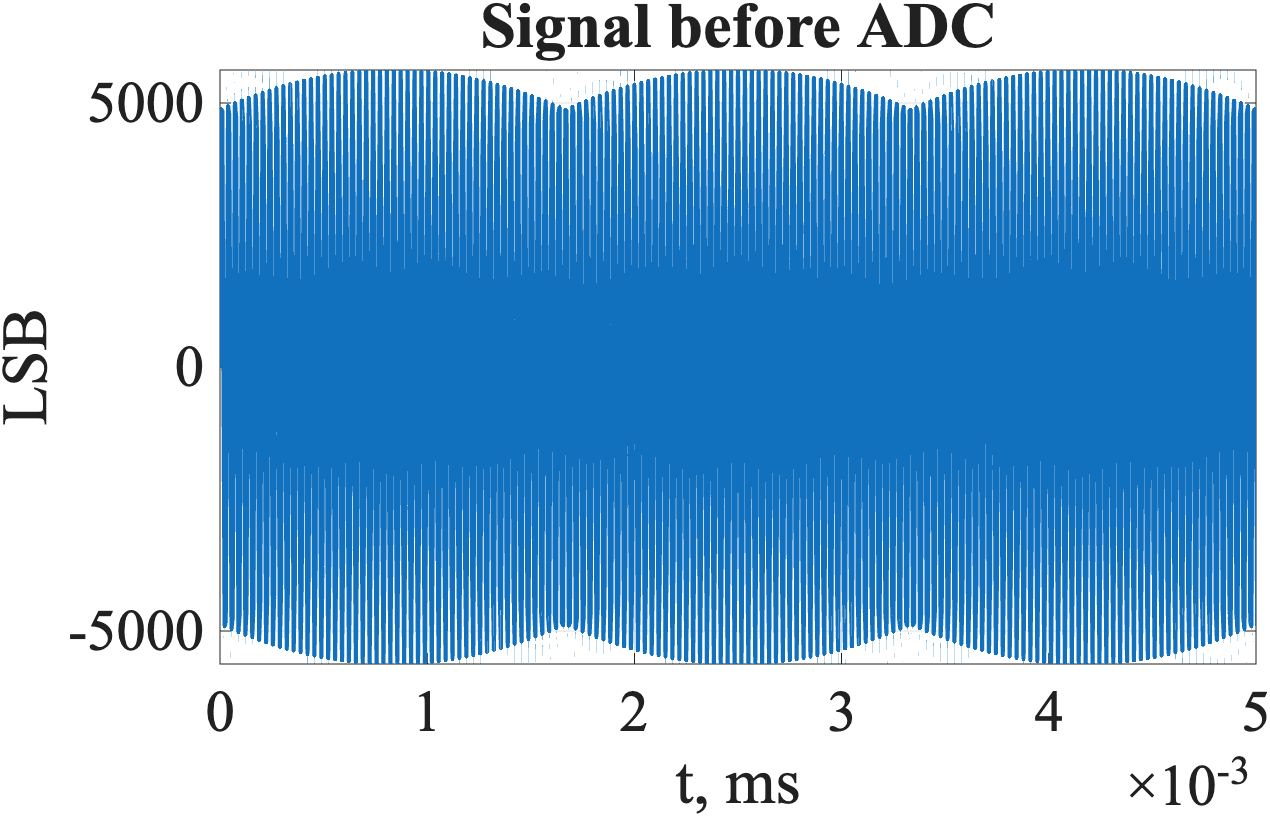
\includegraphics[width=\linewidth]{2_1.png}
        \caption{Входной сигнал до АЦП}
        \label{fig:2_1}
    \end{minipage}
    \hfill
    \begin{minipage}[b]{0.48\textwidth}
        \centering
        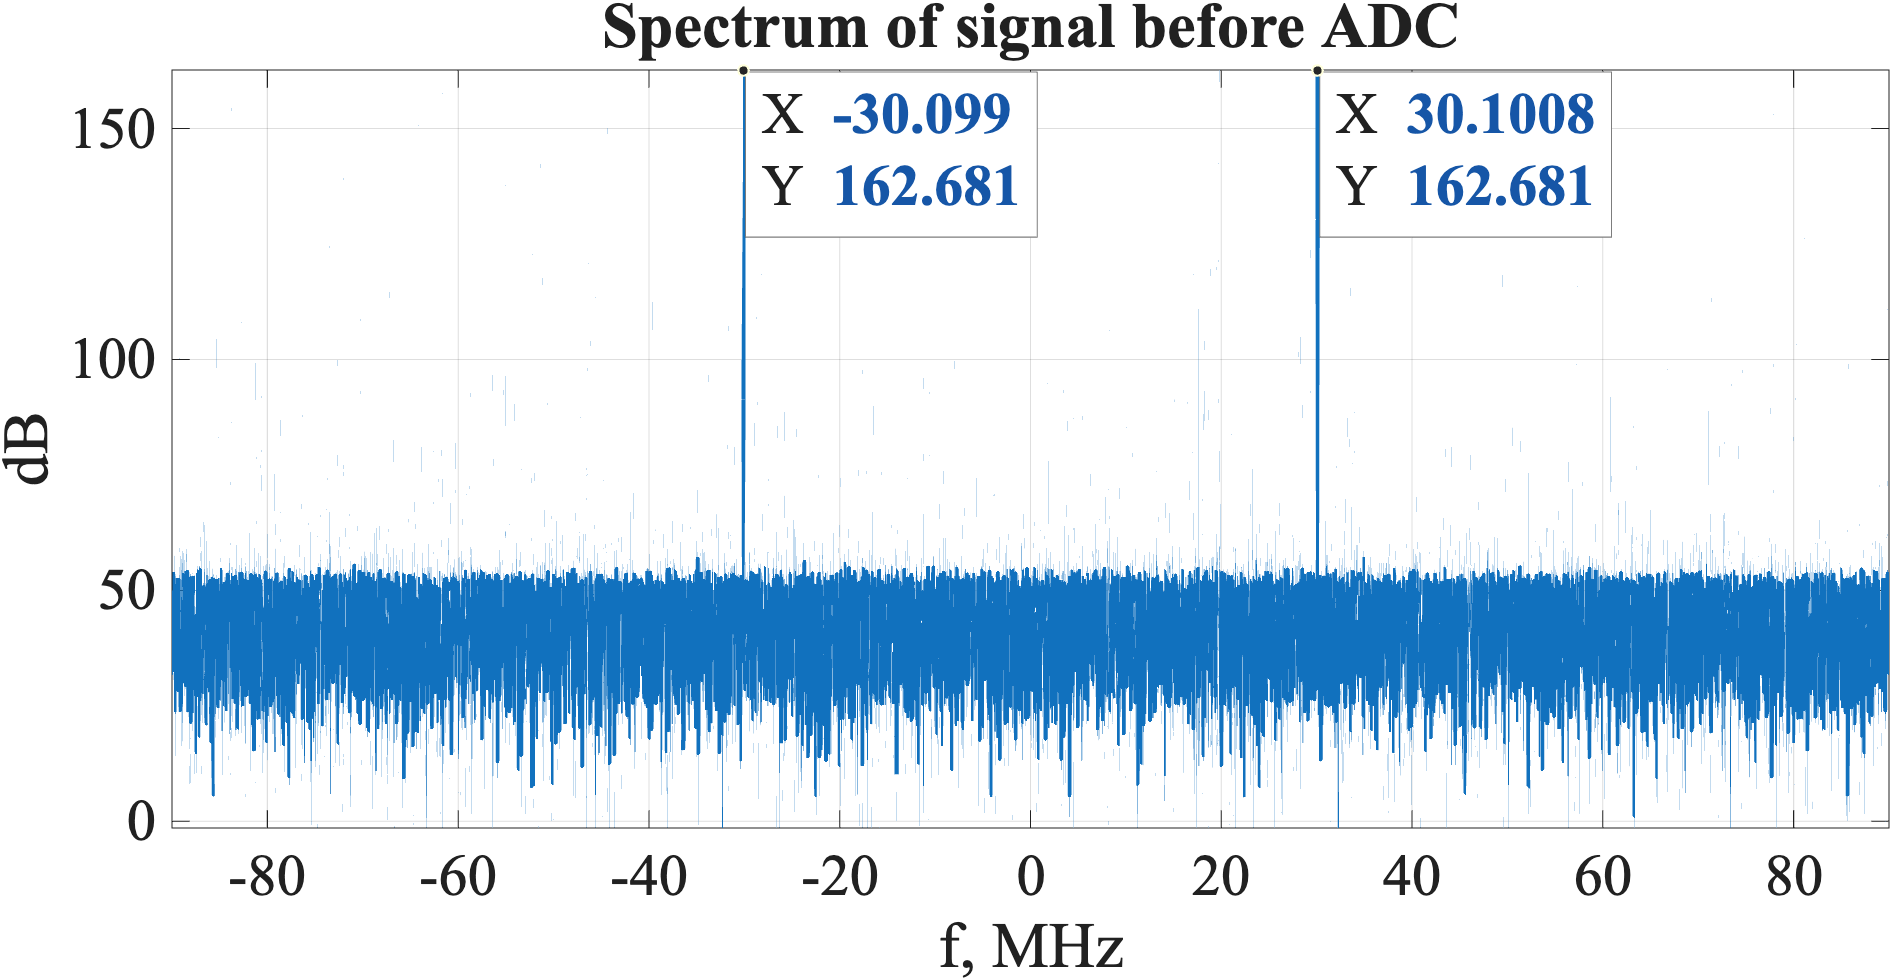
\includegraphics[width=\linewidth]{2_2.png}
        \caption{Спектр входного сигнала}
        \label{fig:2_2}
    \end{minipage}
\end{figure}

На рисунках \ref{fig:2_1} и \ref{fig:2_2} показан исходный аналоговый сигнал, представляющий собой аддитивную смесь монохроматического колебания с частотой $f_C = 210{,}1$~МГц и белого гауссова шума. В скрипте данная смесь формируется путем сложения полезного сигнала \texttt{signal} и шумовой компоненты \texttt{noise}, мощность которой определяется параметром \texttt{snr}. Спектр демонстрирует наличие выраженных спектральных пиков на несущей частоте и равномерный шумовой пьедестал.

% --- Блок 2: Сигнал и спектр после АЦП ---
\begin{figure}[H]
    \centering
    \begin{minipage}[t]{0.48\textwidth}
        \centering
        
\includegraphics[width=\linewidth]{2_3.png}
        \caption{Сигнал после АЦП}
        \label{fig:2_3}
    \end{minipage}
    \hfill
    \begin{minipage}[t]{0.48\textwidth}
        \centering
        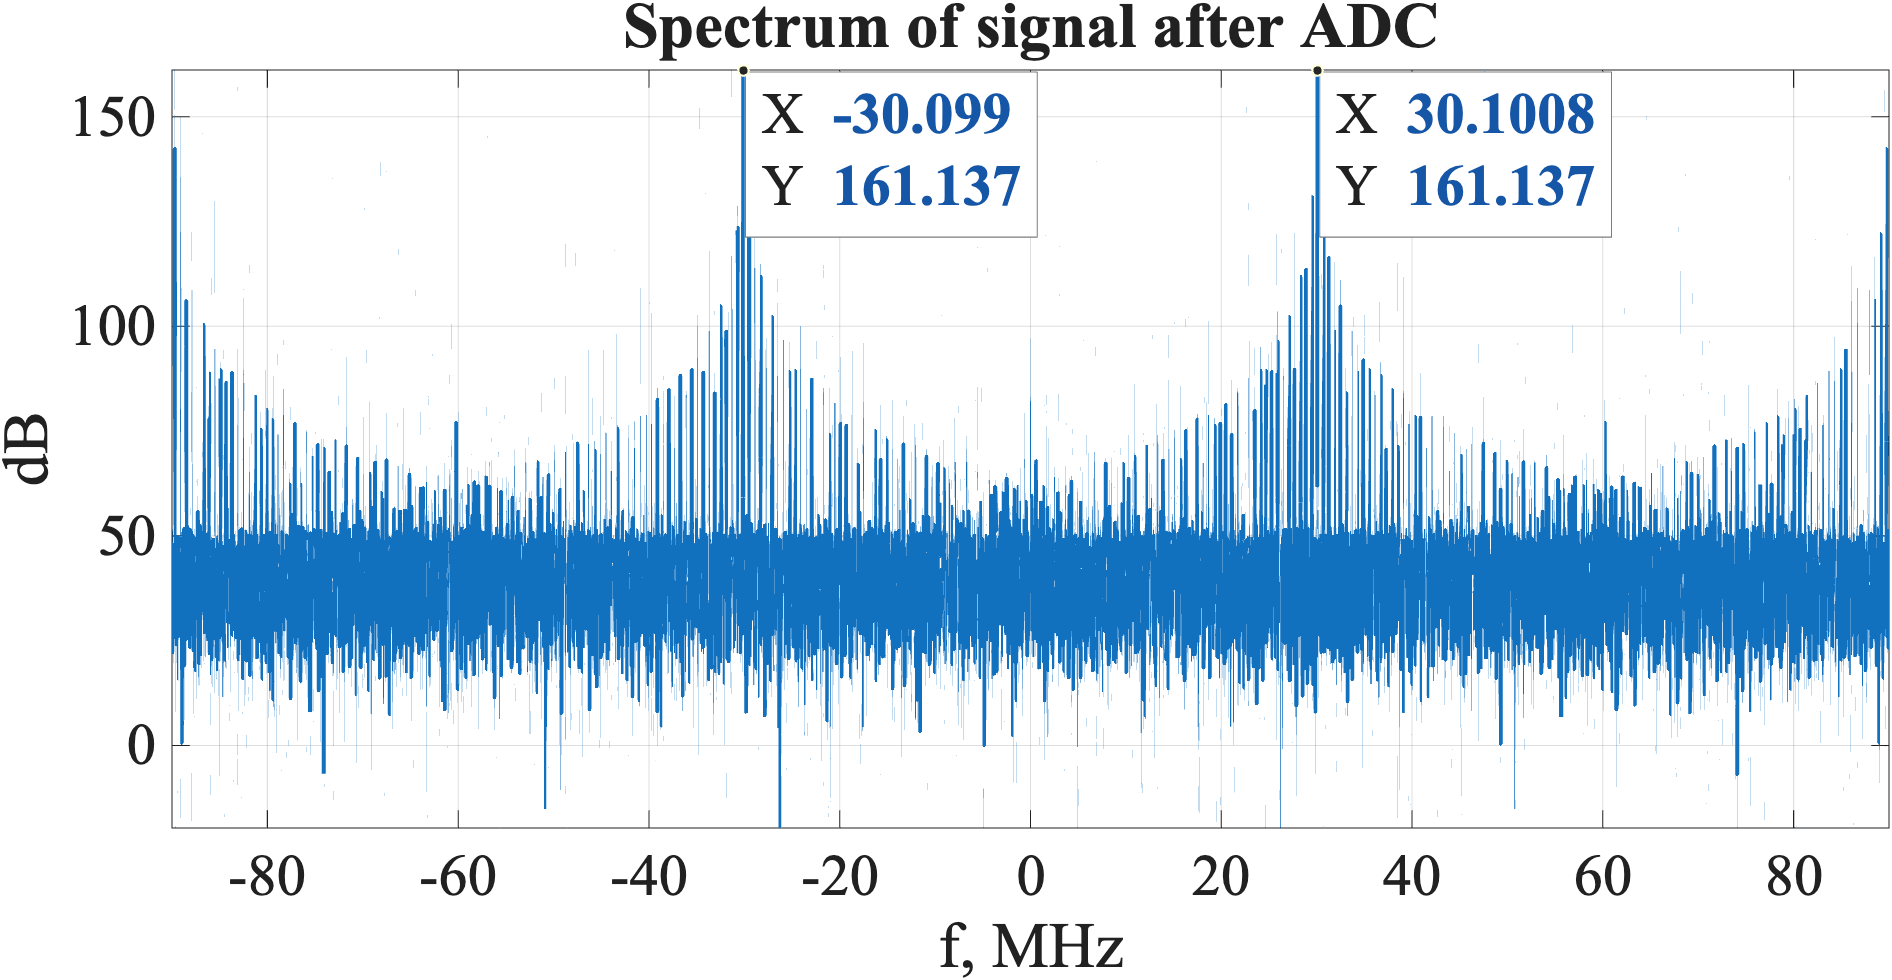
\includegraphics[width=\linewidth]{2_4.png}
        \caption{Спектр сигнала после АЦП}
        \label{fig:2_4}
    \end{minipage}
\end{figure}
Рисунки \ref{fig:2_3} и \ref{fig:2_4} иллюстрируют результат аналого-цифрового преобразования с частотой дискретизации $f_S = 180$~МГц и разрядностью $n_a = 13$~бит. Поскольку частота входного сигнала $f_C = 210{,}1$~МГц превышает половину частоты дискретизации ($f_S/2 = 90$~МГц), возникает эффект субдискретизационного преобразования (алиасинга). Полезный сигнал зеркально переносится в первую зону Найквиста на алиасинговую частоту:
$$f_{\text{alias}} = |f_C - f_S| = |210{,}1 - 180| = 30{,}1 \text{ МГц}$$
Процесс квантования, реализуемый в скрипте функцией \texttt{get\_adc}, математически можно описать выражением:
$$s_{\text{adc}}[n] = Q_{n_a} \{ s(n T_S) + \text{noise}(n T_S) \}$$
где $Q_{n_a}$ — оператор квантования, выполняющий округление вниз (\texttt{Floor}) с ограничением переполнения (\texttt{Saturate}) до 13 бит.
% --- Блок 3: Сигнал и спектр цифрового гетеродина ---
\begin{figure}[H]
    \centering
    \begin{minipage}[t]{0.48\textwidth}
        \centering
        
\includegraphics[width=\linewidth]{2_5.png}
        \caption{Сигнал на выходе ЦГ}
        \label{fig:2_5}
    \end{minipage}
    \hfill
    \begin{minipage}[t]{0.48\textwidth}
        \centering
        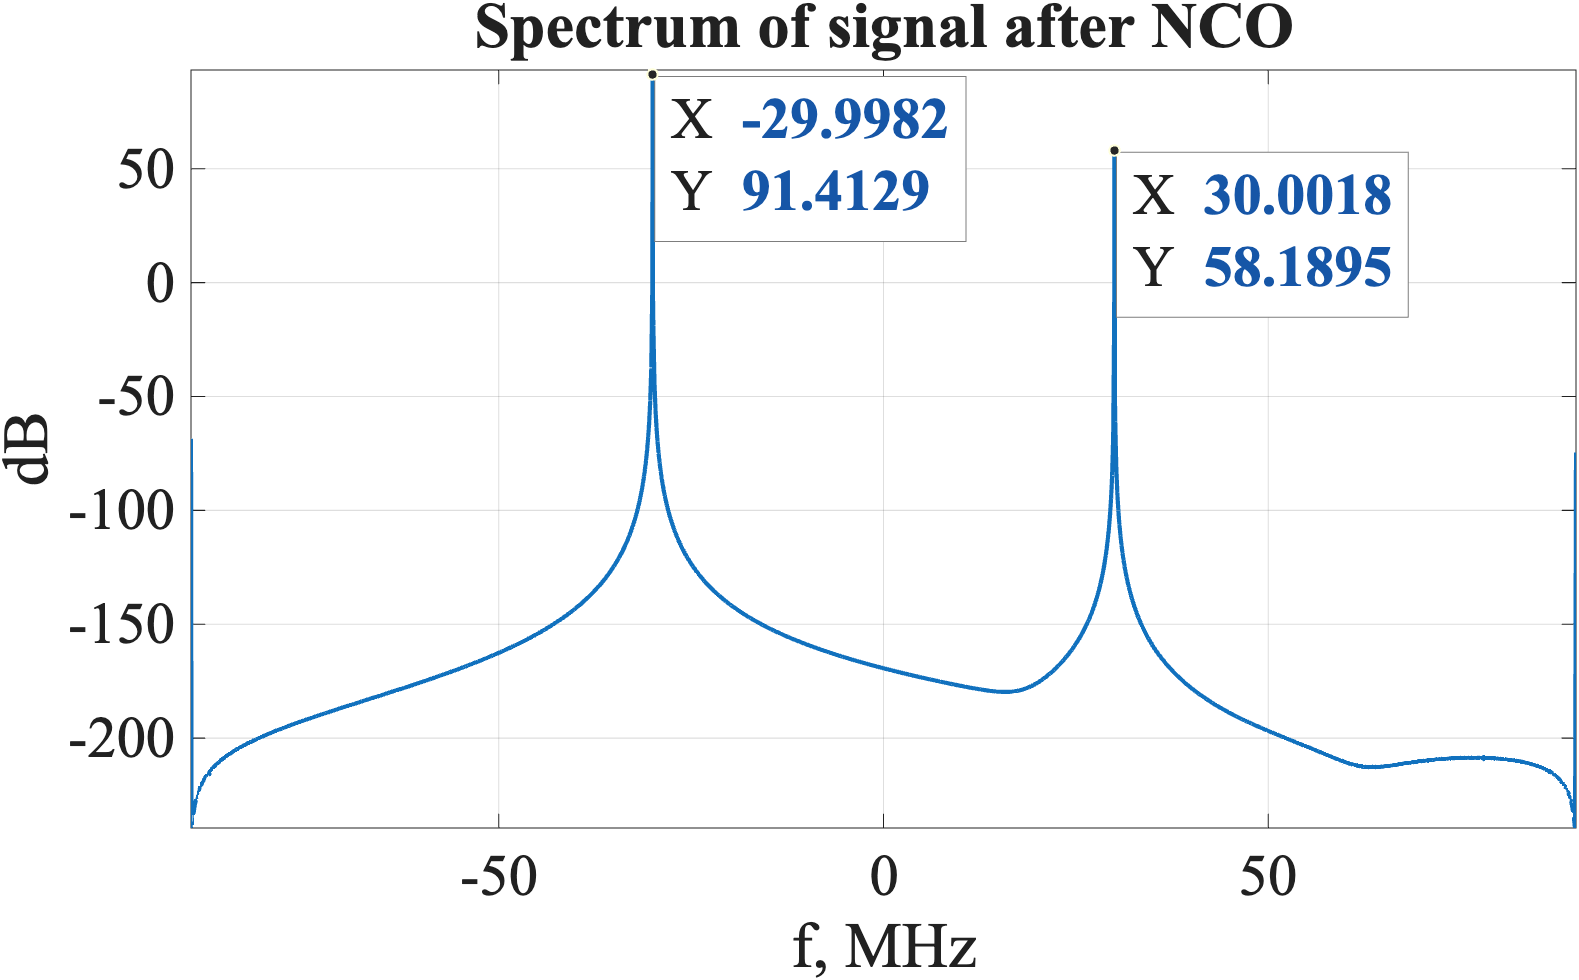
\includegraphics[width=\linewidth]{2_6.png}
        \caption{Спектр сигнала ЦГ}
        \label{fig:2_6}
    \end{minipage}
\end{figure}

% На рисунках \ref{fig:2_5} и \ref{fig:2_6} отображены квадратурные компоненты цифрового гетеродина, настроенного на частоту $f_G = 210$~МГц. Как и входной сигнал, опорное колебание алиасится к частоте $30$~МГц. В функции \texttt{get\_nco} задан фазовый разбаланс \texttt{pmv = 2} градуса. Из-за неидеальной ортогональности I и Q каналов подавление зеркальной спектральной составляющей оказывается неполным, что отчетливо видно в виде симметричного паразитного пика в спектре гетеродина.
На рисунках \ref{fig:2_5} и \ref{fig:2_6} отображены квадратурные компоненты цифрового гетеродина, настроенного на частоту $f_G = 210$~МГц. Как и входной сигнал, опорное колебание подвергается алиасингу, однако переносится на частоту $30{,}0$~МГц. Формирование ортогональных отсчетов в функции \texttt{get\_nco} с учетом заданных искажений происходит по следующим аналитическим выражениям:
$$I[n] = 10^{\frac{\text{amv}}{20}} \cdot \cos(2\pi f_G n T_S)$$
$$Q[n] = \sin(2\pi f_G n T_S + \Delta\phi)$$
В данном базовом прогоне задан начальный фазовый разбаланс $\Delta\phi = \text{pmv} = 2^\circ$. Из-за неидеальной ортогональности $I$ и $Q$ каналов подавление зеркальной спектральной составляющей оказывается неполным, что отчетливо видно в виде симметричного паразитного пика в спектре гетеродина.

% --- Блок 4: Сигнал и спектр после демодулятора ---
\begin{figure}[H]
    \centering
    \begin{minipage}[t]{0.48\textwidth}
        \centering
        
\includegraphics[width=\linewidth]{2_7.png}
        \caption{Квадратуры на выходе DEM}
        \label{fig:2_7}
    \end{minipage}
    \hfill
    \begin{minipage}[t]{0.48\textwidth}
        \centering
        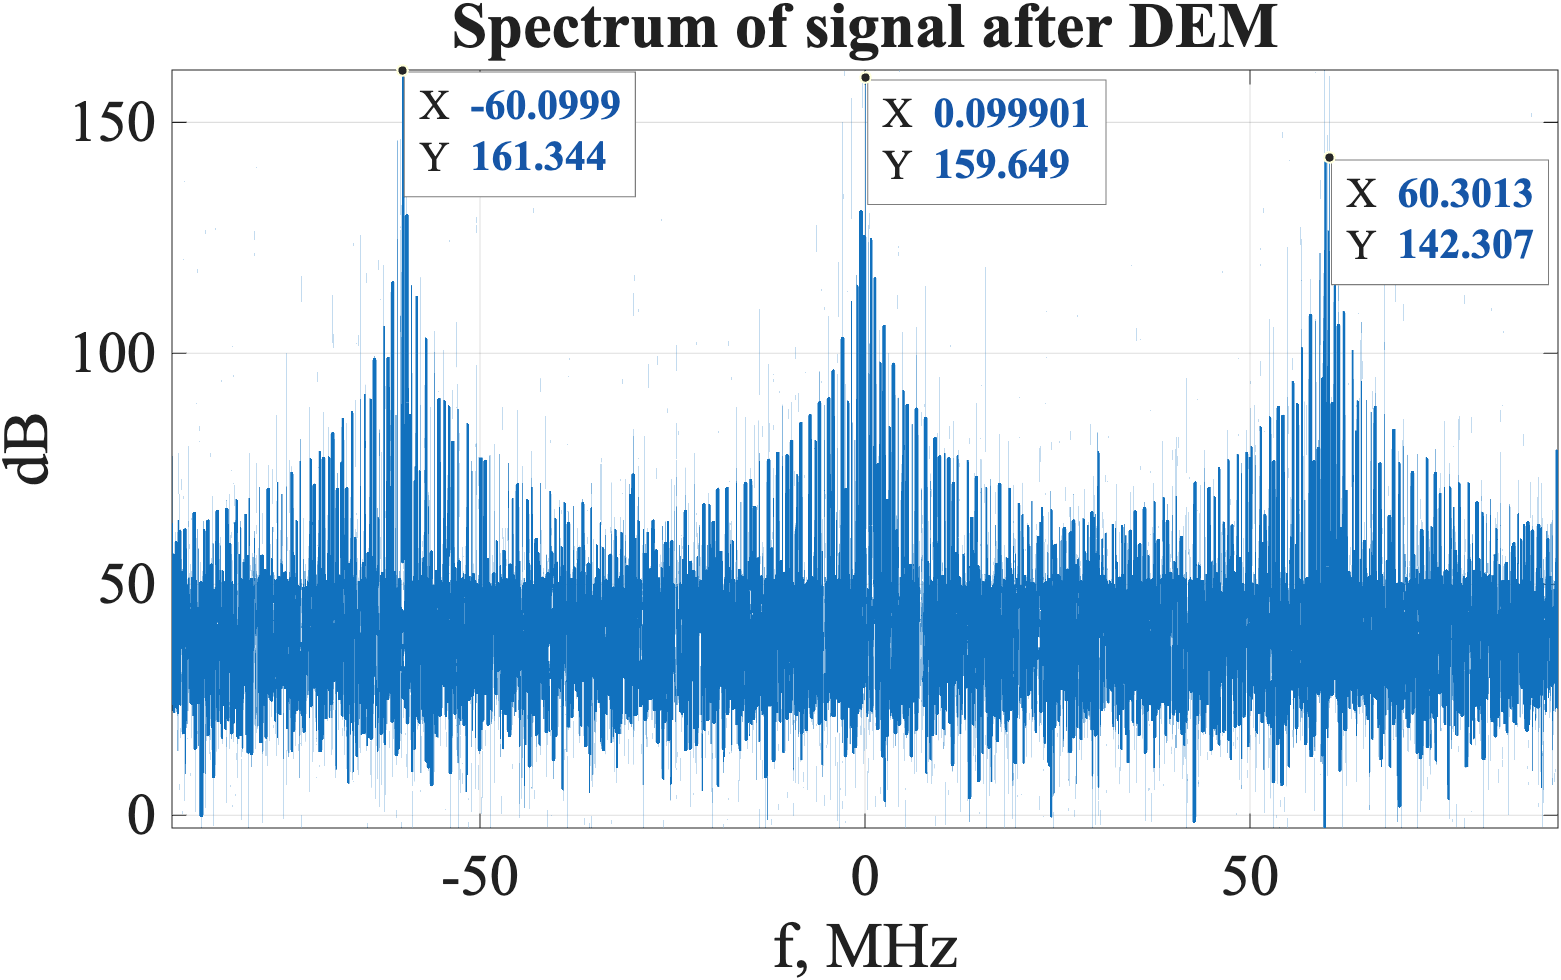
\includegraphics[width=\linewidth]{2_8.png}
        \caption{Спектр на выходе DEM}
        \label{fig:2_8}
    \end{minipage}
\end{figure}

Рисунки \ref{fig:2_7} и \ref{fig:2_8} демонстрируют результат работы цифрового демодулятора, реализованного в коде функцией \texttt{get\_dem} путем перемножения отсчетов сигнала с АЦП и комплексных отсчетов ЦГ. В результате гетеродинирования спектр сдвигается на нулевую частоту. Благодаря заложенной отстройке в $0{,}1$~МГц ($210{,}1 - 210{,}0$), во временной области наблюдается низкочастотное биение. В спектре доминирует пик на частоте $0{,}1$~МГц, однако из-за фазовых искажений ЦГ присутствуют зеркальные побочные спектральные составляющие, снижающие динамический диапазон приемника.
В результате комплексного перемножения спектр сдвигается к нулевой частоте. Возникающая разность частот между алиасной частотой сигнала ($30{,}1$~МГц) и алиасной частотой гетеродина ($30{,}0$~МГц) формирует на выходе демодулятора низкочастотное биение:
$$f_{\text{out}} = f_{\text{alias\_sig}} - f_{\text{alias\_nco}} = 30{,}1 - 30{,}0 = 0{,}1 \text{ МГц}$$
В спектре доминирует пик на частоте $0{,}1$~МГц, однако из-за фазовых искажений ЦГ...
